%%%%%%%%%%%%%%%%%%%%%%%%%%%%%%%%%%%%%%%%%%%%%%%%%%%%%%%%%%%%%%%%%%%%%%%%%%%%
% FILE    : ToolsLibraries.tex
% SUBJECT : Document describing the tools and libraries used by VTank.
% AUTHOR  : (C) Copyright 2010 by Vermont Technical College
%
%%%%%%%%%%%%%%%%%%%%%%%%%%%%%%%%%%%%%%%%%%%%%%%%%%%%%%%%%%%%%%%%%%%%%%%%%%%%

\chapter{Tools and Libraries}
\label{toolslibraries}

This chapter describes the tools and libraries used in the \VTank\ development environment. Both where to get the necessary components and how to set them up are covered here. This chapter is only of interest to \VTank\ developers. If you are a \VTank\ player or administrator you do not need to read this chapter. Instead the details for setting up the components of a working \VTank\ system are described in Chapter~\ref{deployment} on Deployment.

The following list reflects the tools and libraries used by the \VTank\ developers. \pcnote{We should elaborate on how to set up and configure these tools and libraries as appropriate. Probably each tool and library should eventually be put into its own section.}

\begin{itemize}
\item Visual Studio 2008
\item Stackless Python
\item XNA Framework v\XNAVersion
\item DirectX SDK \DirectXSDKVersion
\item Threadpool \cite{threadpool}
\item Ice v3.4.1 \cite{ice}
\item Dia \cite{dia}
\item MySQL
\item NUnit
\item xWinForms
\item NSIS
\item XACT
\item Dynamic Model Viewer
\item Map Previewer
\end{itemize}

\section{Boost}

Boost is an advanced collection of C++ libraries originally intended as a testing ground for facilities that might one day become part of the C++ standard \cite{boost}. The libraries in Boost are peer reviewed and are generally of high quality. They also take advantage of many advanced C++ features to provide a degree of elegance one rarely finds in ordinary C++ libraries.

The \VTank\ project uses Boost freely in the two C++ projects, \GameServer\ and \MapEditor. Building either of these projects requires that you install Boost. Developing either of these projects requires that you be familiar with at least some of the Boost libraries such as \lstinline!boost::smart_ptr! and \lstinline!boost::thread!.

The official version of Boost used by the \VTank\ project is version \BoostVersion. Other nearby versions are likely to work; many Boost libraries do not change much between versions. Of course for maximum compatibility with the existing \VTank\ code base we recommend that you install precisely version \BoostVersion.

Many of the Boost libraries are expressed as templates and thus are entirely contained in their header files. These libraries do not need to be explicitly compiled. They are effectively compiled each time the header files are included. However some Boost libraries, notability \lstinline!boost::thread! and \lstinline!boost::regex!, do have supporting implementation files that need to be compiled separately.

While it may be possible to download compiled Boost binaries for Windows or Linux (for example using your Linux distribution's package manager), we recommend building Boost from scratch. Ultimately this gives you more control over the configuration of the library and it ensures that the library as built corresponds properly to the other tools and libraries you are using. We give a summary of the build instructions, with \VTank\ related notes, below. Note that we currently only describe the build on Windows. Linux development is not officially supported, but it should be easy to adapt these instructions for that environment as well.

\subsection{Windows}

To build Boost perform the following steps.

\begin{enumerate}

\item Download the Boost library from the Boost web site \cite{boost}. Unpack it to some suitable location on your system. To satisfy \VTank\ build requirements you will need to set the BOOSTROOT environment variable to point at this location. We recommend that you make this a system environment variable and reboot your machine to ensure that it takes effect globally before trying to build \VTank. Note, however, that BOOSTROOT is not required by Boost itself and so you can continue building Boost (below) without it.

\item Open a Visual Studio command prompt so that access to the Visual C++ command line tools is available.

\item In the root of the Boost source tree (\%BOOSTROOT\%) execute the command
\begin{commands}
bootstrap
\end{commands}

This command builds the \command{bjam} tool used to do the rest of the build. The resulting executable \filename{bjam.exe} is left in \%BOOSTROOT\%.

\item Use \command{bjam} to build the various libraries you need. For example, to build the \lstinline!boost::thread! library use the following command
\begin{commands}
.$\backslash$bjam variant=debug,release link=shared,static thread
\end{commands}

This command creates both debug and release variants as both shared libraries (DLLs) and static libraries\footnote{Note that the \lstinline!boost::thread! library also requires the \lstinline!boost::date\_time! library.}. The result of the build is placed under \filename{\%BOOSTROOT\%$\backslash$bin.v2} in a complex folder structure that organizes the different build variations. Note that by default \command{bjam} builds multi-thread enabled libraries. This is desired.

\item Create a folder \filename{\%BOOSTROOT\%$\backslash$lib} to hold the final libraries. This folder makes it more convenient to use the libraries since they will all be in a common location with a relatively short path. Furthermore the \VTank\ build system assumes this configuration. Copy the compiled libraries of interest to this new folder.

\end{enumerate}

It is possible to use \command{bjam} to build all Boost libraries in all variations in one step. However, this generates a very large amount of output and is overkill for \VTank. Also some Boost libraries have additional dependencies and configuration requirements that must be satisfied before they will build successfully. It is easier, and less resource consuming to only build the libraries that are actually needed. You can always use \command{bjam} as above to build other Boost libraries later.

Note that the Boost libraries are named according to a naming convention that distinguishes the library variants from each other. This allows all variants of all libraries to coexist in a single folder. See the Boost documentation for information on the naming convention used with the library files.

\section{wxWidgets}

\subsection{Windows}

The GUI components of \MapEditor\ are handled using the well known wxWidgets library \cite{wxWidgets}. Version 2.8.9 of wxWidgets is the recommended version. Note that the wxWidgets installer only installs the source code of the library. After running the installer it is still necessary to compile the source using Visual C++. The most straightforward way to build the necessary library files is to change to the \filename{build/msw} folder in the wxWidgets distribution and issuing the command\footnote{If you have the QNX development system also installed on your computer, but sure to erase the contents of the MAKEFLAGS environment variable before issuing the \command{nmake} command.}:

\begin{commands}
nmake /f makefile.vc BUILD=debug UNICODE=1
\end{commands}

This command will build the debug static version of wxWidgets with Unicode support. We recommend using Unicode support because it enforces a more rigorous handling of characters and strings. This in turn creates a higher quality application. It will also facilitate creating an international version of \MapEditor\ in the future. Accordingly the various \MapEditor\ build control files assume a Unicode configuration.

You should also build the release version of wxWidgets with the command

\begin{commands}
nmake /f makefile.vc BUILD=release UNICODE=1
\end{commands}

The debug and release versions can coexist without conflict. In fact, the wxWidgets library can be built for multiple compilers simultaneously. Thus if you intend to also use Code::Blocks on \MapEditor, you can compile wxWidgets using the MinGW version of gcc that comes with Code::Blocks in addition to using VS2008\footnote{Although not a supported configuration you can most likely develop \MapEditor\ using Code::Blocks on Windows. See the supplementary document \filename{CodeBlocks-on-Windows.txt} for more information.}.

You may install wxWidgets anywhere you like. However, the VS2008 project file provided with \MapEditor\ assumes that you have set an environment variable named WXROOT that points to the top folder of your wxWidgets installation. Note that this environment variable is not a required part of the wxWidgets installation; it exists only for \MapEditor\ project files.

\subsection{Linux}

\MapEditor\ development is supported on Linux using gcc. However, because of the large variation in Linux systems, no single set of instructions is likely to be appropriate for all possible Linux distributions. Use the instructions here as a guide. You may have to make some significant changes to them in order to get everything working on your particular system.

Both \MapEditor\ and the Code::Blocks IDE require wxWidgets. It is not essential that they use the same version of wxWidgets, but you may find it convenient for them to do so (especially if you are installing both wxWidgets and Code::Blocks manually). These instructions assume such a configuration.

You may be able to install either or both of wxWidgets and Code::Blocks using your distribution's package manager. There are advantages to taking such an approach. However, if you are interested in developing \VTank, we recommend that you compile both products from source. This will give you more control over their configuration and allow you to use precisely the same versions as the other \VTank developers. In the long run, this will simplify your development. The following steps describe what must be done to manually set up wxWidgets on a typical Linux system.

\begin{enumerate}

\item Download \filename{wxGTK-2.8.9.tar.gz} from the wxWidgets web site. Unpack it in a suitable location (for example, \filename{/usr/local/src}).

\item Follow the installation instructions in \filename{install-gtk.txt}. Basically this entails creating a \filename{buildgtk} subdirectory and then, inside that subdirectory configure as follows:

\begin{commands}
../configure -with-gtk --enable-unicode --enable-monolithic
\end{commands}

The \command{--enable-unicode} and \command{--enable-monolithic} options are both needed by Code::Blocks and \MapEditor.

\item After configuring, do \command{make} and then \command{make install}. The installation will be put into \filename{/usr/local/include} and \filename{/usr/local/lib}, etc.

\item Repeat the procedure in step \#2 except using a \filename{buildgtkd} subdirectory. Add \command{--enable-debug} to the configure command line. This creates the debugging version of the library. When you issue \command{make install} the debugging library will be installed alongside the non-debugging library. The two libraries can coexist.

\item Run the \command{ldconfig} tool to build a new shared library cache reflecting the additions you just made.

\end{enumerate}

NOTE: If you do make install on the release version of wxWidgets and then the debug version, it will be the debug version of the \command{wx-config} helper program that is actually installed. This means that wxWidgets projects that use \command{wx-config} will end up building against the debug version of the wxWidgets library. This may or may not be desirable. For example it turns out that Code::Blocks v8.02 does not work with the debugging wxWidgets library. You may wish to install the debugging version of wxWidgets first so that the final version of \command{wx-config} is actually the release version.

Using wxWidgets in Code::Blocks projects is actually fairly simple. To access the headers use the string \command{`wx-config --cflags`} (note back quotes) in the `Other Options' tab of the `Compiler Settings' tab of the build options dialog. To access the libraries use the string \command{`wx-config --libs`} (note back quotes) in the `Other Linker Options' box of the `Linker Settings' tab of the build options dialog. You can make these changes at the top level of the options definition. There is no need to specialize for debug and release builds. However, be aware that this means both the debug and release versions of your program will be using whichever version of wxWidgets is reported by \command{wx-config} (see the previous paragraph for more on this issue).

\section{CruiseControl.NET}

Note that if you install IIS after installing the .NET Framework you will need to explicitly install ASP.NET v2 into your IIS system. The IIS installer does not do this automatically\footnote{However, the .NET Framework installer will install ASP.NET into your IIS system if IIS is already installed when the .NET Framework is installed.}. To take care of this detail manually, open a VS2008 command prompt (this assumes you have Visual Studio installed already) and issue the command

\begin{commands}
aspnet\_regiis -i
\end{commands}

The C++ components of \VTank\ use a custom unit test framework. You will need to configure CC.NET in a special way before it will understand how to execute and display the unit tests that use this framework. Specifically, in the CC.NET configuration file, inside the sections for the \GameServer\ and \MapEditor\ projects, include the following \xml{exec} task immediately after the \xml{msbuild} task.
\begin{verbatim}
<exec>
  <executable>check.exe</executable>
  <baseDirectory>Debug</baseDirectory>
  <buildArgs>check.xml</buildArgs>
</exec>
\end{verbatim}

It is important to include this task after the \xml{msbuild} task so that it executes only if the \xml{msbuild} task executes first and completes successfully.

Next in the \xml{publishers} section immediately before any XML logger tasks include the following
\begin{verbatim}
<merge>
  <files>
    <file>Debug\check.xml</file>
  </files>
</merge>
\end{verbatim}

This will combine the unit test results into CC.NET's overall build log where they can be subsequently analyzed and displayed.

Finally, in order for the results of the unit tests to be displayed properly on the web dashboard it is necessary to install an appropriate XSL file into the web dashboard's configuration. In the root of the web dashboard application, edit the file \filename{dashboard.conf}. In the \xml{buildReportBuildPlugin} element, add an \xml{xslFile} child element that names \filename{UnitTestManager.xsl}. Copy this file into the \filename{xsl} subfolder. Note that the existing reference to \filename{unittests.xsl} should not be removed. That XSL file formats the test output from NUnit or JUnit. Since this configuration change applies to all projects and since some \VTank\ projects use NUnit, it is necessary for both unit test formatting transformations to be present.

It might be desirable at some point to configure the dashboard so that each project has unique settings for the \xml{buildReportBuildPlugin} element. With the configuration described here it is necessary to ignore one of the unit test sections in each project (both are always displayed even though only one is used per project).

Note that it is necessary to restart IIS after changing \filename{dashboard.conf} in order for the changes to take effect.

\subsection{Creation of a Client}

The \VTank build script creates a new release client every time there is a successful build. Five main steps accomplish this task. 
\begin{enumerate}

\item Build Release version of the VTank
\item Kill the IcePatch2 server via PSKill
\item Update the new \Client\ files via the script UpdateClientFiles.bat
\item Build a new distribution of Patcher files via MakePatcherDistribution.bat
\item Restart the IcePatch2 server

\end{enumerate}

These are all run in order in our build script, as to make sure corrupt files don't make their way to the customer via the patcher.

\section{\LaTeX}

The primary \VTank\ documentation is written using the \LaTeX\ typesetting system \cite{latex}. This system provides high quality output with an input format that is friendly to software development tools and methods. All \VTank\ developers are expected to have some familiarity with \LaTeX\ so that they will feel comfortable editing the documentation as their work unfolds.

Although it is likely that the \VTank\ documentation could be compiled as-is on a Linux system with \LaTeX\ installed, we assume that all documentation will be edited on Windows using the MiKTeX version \MiKTeXVersion\ \cite{miktex}. Installation of MiKTeX is straight forward and essentially entails downloading the installer and running it. Here are a few notes about this process.

\begin{enumerate}

\item MiKTeX can be installed in a manner where it downloads packages on demand as they are first used. This approach minimizes the amount of disk space initially used by the system with the disadvantage of requiring Internet access when compiling a document that uses a new package for the first time. Alternatively one can do a ``complete'' installation where all packages are installed initially. This consumes a lot of disk space but it also means that any document can be compiled at any time without Internet connectivity.

\item It is convenient to include the MiKTeX bin folder on your path. This folder is
\begin{commands}
C:$\backslash$Program Files$\backslash$MiKTeX 2.7$\backslash$miktex$\backslash$bin
\end{commands}

This allows you to execute the various \LaTeX\ compilers and associated tools from the command line if desired. Some \LaTeX\ aware editors assume this ability in order to compile documents for you. Note that the MiKTeX installer may automatically take care of setting up your path for you.

\item It is probably a good idea to get in the habit of updating your MiKTeX installation periodically. From the Start Menu go to ``MiKTeX 2.7'' and then ``Update.'' The updater will identify packages that are available for updating and automatically download and install them.

\item On some machines at some times the installation or update of MiKTeX fails with a message like ``unable to write to the cache.'' This message is (most likely) from \command{fc-cache}, a tool used to create the font cache for \command{xetex}. If you are not using \command{xetex} (and \VTank\ does not) you can ignore this error. However, you can also try executing \command{fc-cache} from the command prompt manually. This often corrects the problem (the issue appears to be related to the execution of \command{fc-cache} under the control of the installation utility). For example
\begin{commands}
fc-cache -f -v
\end{commands}
The community appears to be uncertain as to why this problem occurs.

\end{enumerate}

In addition to \LaTeX\ itself you will also want to install a \LaTeX\ editing environment. In theory you can use any text editor. In fact many editors (Emacs, Notepad++, etc) have special \LaTeX\ editing modes to make the preparation of \LaTeX\ documents easier. However, the official \VTank\ environment for editing \LaTeX\ documents is TeXnicCenter version \TeXnicCenterVersion\ \cite{texniccenter}. This program provides an IDE-like environment for working on \LaTeX\ documents, complete with a project facility and many menu items for selecting various \LaTeX\ environments and features.

The installation of TeXnicCenter is straight forward. Note, however, that you should install MiKTeX first so that TeXnicCenter can auto-detect it and configure itself appropriately. If you install TeXnicCenter first, you will need to manually configure the various output profiles later.

The use of TeXnicCenter is mostly self evident. To edit the \VTank\ documentation, open the file \filename{VTank.tcp} in the \filename{Docs} folder. This is the TeXnicCenter project file for the \VTank\ documentation. From here you can navigate to the other files as needed and build the final PDF by clicking on the ``build output'' button on the top TeXnicCenter tool bar (it's near the center).

MiKTeX comes with the necessary tools out of the box to build PDF and PostScript output. To view this output you will need a PDF viewer and a PostScript viewer. Note that at this time the \VTank\ documentation only requires PDF tools. However, you may wish to install PostScript support as well for other \LaTeX\ projects.

The widely used Acrobat PDF viewer works perfectly well, but you may want to consider a different viewer that does not hold the PDF file open all the time. This allows you to keep the document on display while you compile a new version of the document. With Acrobat, the compilation will fail if Acrobat is displaying the file because Acrobat locks the file. A viewer that works better in this situation is SumatraPDF (it is also open source).

The open source Ghostscript and its associated viewer GSView work well for displaying PostScript files.

 
\section{PC-Lint}

PC-Lint is a commercial static analysis tool for C++ by Gimpel Software \cite{pc-lint}. At the time of this writing the \VTank\ developers are using the latest patch release of PC-Lint version \PCLintVersion, applying the tool to the two C++ projects in VTank: \GameServer\ and \MapEditor.

PC-Lint is very configurable and, in fact, creating the detailed configuration files needed by the tool is a considerable amount of work. Thus the precise PC-Lint configuration used with \VTank\ is checked into the repository where it can evolve along with the rest of the code base. Although the PC-Lint installer will help you set up a default configuration, this is useful only if you intend to apply PC-Lint to other projects. The configuration created by the installer is ignored when you apply PC-Lint to \VTank.

In each folder where PC-Lint can be used the file \filename{LIN.BAT} runs PC-Lint assuming that it has been installed in the default location. However, it directs PC-Lint to \VTank\ specific configuration files. The \filename{lint-config} folder off the root of the \VTank\ source tree contains general configuration information that applies to all \VTank\ projects. Note that in \filename{lint-config} the files \filename{options.lnt} and \filename{std.lnt} contain \VTank\ customizations. All other files in that folder are intended to be identical to those provided in the PC-Lint distribution.

In addition, \filename{LIN.BAT} includes a project specific configuration file that is customized for each \VTank\ project. For example the project specific configuration for \MapEditor\ is in \filename{Map\_Editor.lnt} in the \MapEditor\ root folder. In most cases, adjustments to the PC-Lint configuration should be done in this project specific file. This allows individual \VTank\ projects to use PC-Lint to enforce different polices. The project specific configuration is also the appropriate place to include annotations about project specific functions.

In addition each project contains a file containing a list of linted source files. For example the file list for \MapEditor\ is in \filename{Map\_Editor-FileList.lnt} in the \MapEditor\ root folder. This file can be given as an argument to \filename{LIN.BAT} to direct PC-Lint to process the entire program in one run. This is necessary to take advantage of PC-Lint's inter-module analysis. It is also possible to execute \filename{LIN.BAT} on one source file at a time. This would be the usual approach during development when changes to one file need to be checked.

\subsection{Usage Notes}

\VTank\ uses PC-Lint in a fairly strict mode of operation. The tool thus produces many messages when applied to ``ordinary'' C++ code. To make the burden of using PC-Lint manageable it is important to apply the tool frequently to developing code and to address the messages it produces as soon as possible. This minimizes the number of messages produced in any one run of the tool.

The ultimate goal is to evolve a PC-Lint configuration that is both strict and precise. The configuration should be strict in the sense that it should detect many common problems and force the \VTank\ developers to use good C++ programming style. The configuration should be precise in the sense that it should, to the greatest extent possible, capture complete and correct semantic information about the functions used. This will allow PC-Lint to detect real errors that would go unnoticed by an ordinary compiler.

Since building an appropriate PC-Lint configuration is itself a non-trivial undertaking, it is expected that it will take some time before that configuration is in its final state. As both the code and configuration change, the amount of output produced by PC-Lint will naturally fluctuate. Thus while it is desirable to create code that is completely ``lint free,'' it is also expected that developers will sometimes check in code that contains lint.

\emph{It is important that developers do not rush to eliminate PC-Lint output by simply disabling messages.} Often the significance of a message is not immediately obvious. What's more, when the meaning is clear it is often not immediately obvious what the best fix might be. In many cases, PC-Lint messages indicate deep design and organizational problems that go well beyond the immediate issue being diagnosed. Applying a ``quick fix'' solution, especially by disabling the message in question, will negate many of the benefits of using the tool.

\section{Ice-\IceVersion}

Ice binaries are available for download at \url{http://zeroc.com}.

\subsubsection*{Windows}

Download the latest installer package for Visual Studio 2008. Install the package and make a note of where it's installed. Set the environment variable \command{ICEROOT} to the location where Ice was installed (information on how to do that is not covered in this document). Some compile scripts use the \command{ICEROOT} variable to locate certain binary or required slice files.

If it installed correctly, a new plug-in should be available for Visual Studio 2008 which allows you to configure Ice. Most of the instructions below are for administrators who are configuring Ice from scratch. However, it's important (and necessary) to go through and make sure your configuration mirrors this document's configuration.

Right-click on any project which uses Ice (e.g. the Network project), and at the bottom of the pop-up menu you should see ``Ice Configuration...''. Selecting the ``Ice Configuration...'' option should bring up the option dialog to configure Ice for that project. Every project which uses Ice in some way must be configured like so:

\begin{itemize}
  \item Set the ``Ice Home'' field to ``\command{\$(ICEROOT)}'' (without the quotation marks).
  \item Under the ``Ice Components'' section, check the 'Ice', 'Glacier2', and 'IceSSL' fields at the bottom. This will add assembly references to these DLLs to the project.
  \item Click the ``Close'' button.
\end{itemize}

These instructions are slightly different for two projects in particular: the IceCs project and the IceCpp project. In \emph{both} of those projects, ensure the following configurations are set:

\begin{itemize}
	\item Set the ``Ice Home'' field to ``\command{\$(ICEROOT)}'' (without the quotation marks).
	\item Under the ``Slice Compiler Options'', check the ``Streaming'' box. \emph{Note: this must be checked due to a bug in Ice 3.4.0. This bug has been patched by ZeroC and is expected to be incorporated into Ice 3.4.1}.
	\item Under the ``Slice Include Path'', click ``Add''. Simply type a period (i.e. the current directory) and press Enter. Ensure that the check box which appears after you press Enter is unchecked.
	\item Under the ``Ice Components'' section, check the 'Ice', 'Glacier2', and 'IceSSL' fields at the bottom. This will add references to these assembly DLLs to the project.
\end{itemize}

You will know if every project which uses Ice is not configured properly because it will complain about missing assembly references to Ice or Glacier2. If that occurs, check the project which reports this error, then ensure that project's Ice configuration is correct.

\subsubsection*{Ice with Python}

The following instructions were tested with Python 2.6.4. It is not guaranteed to work the same in any other versions. 

Edit the \command{PYTHONPATH} environment variable to include the following paths:

\begin{itemize}
	\item \%ICEROOT\%\verb+\+bin
	\item \%ICEROOT\%\verb+\+python
\end{itemize}

Note that you may need to use the x64 folder in your paths in the case of a 64 bit operating system:

\begin{itemize}
	\item \%ICEROOT\%\verb+\+bin\verb+\+x64
	\item \%ICEROOT\%\verb+\+python\verb+\+x64
\end{itemize} 

Run the Python interpreter and type:

\command{import Ice;}

You may get an error about a missing DLL. If so, the easiest way to deal with this is to add \command{\%ICEROOT\%/bin} to your \command{PATH} environment variable. Doing so will add the DLLs for Ice to your PATH. The alternate way to deal with this is to copy all of the Ice DLLs into the python/DLLs folder. It's important to remember to restart your terminal or your computer if necessary after making modifications to environment variables.

\subsubsection*{Linux}

\emph{Note: These instructions may not work correctly with VTank. VTank administrators now compile Ice manually on Linux machines. This documentation will be updated in the future.}

Linux machines with \filename{yum} installed can view Ice packages from the Ice repository. ZeroC provides a more detailed explanation regarding exactly how to install and update Ice automatically and from RPM packages at:

\url{http://www.zeroc.com/download.html\#linux\_rpms}

The \filename{yum} installer will install all of the Ice binaries and files required to run Python under the default installation of Python. You may have to compile Ice yourself if you are not using the default installation of Python.

\section{Threadpool}

Threadpool is a third-party addon to the Boost library that leverages the \lstinline!boost::thread! class to create functionality similar to Stackless Python. Each 'thread' in the threadpool is actually a customized task. Rather than creating a separate thread for each task inside of the pool, the tasks are executed in a concurrent fashion. The tasks are not run in parallel to each other. Instead, it uses a scheduler to decide which tasks it should execute and when. Therefore, if a certain set of data is only accessed by one threadpool, it does not require thread safety. Every new threadpool created uses a \lstinline!boost::thread! to run the scheduler.

\subsubsection*{Windows}

Installing the Threadpool library is relatively easy. The project is available on sourceforge at the address: \url{http://threadpool.sourceforge.net}. On the front page, scroll down to the section labelled as `Download Section'. Download the source (the package ending in `src.zip') by clicking on the link.

Threadpool can be extracted anywhere you prefer. In Visual Studio, add the Threadpool include directory and the boost directory that was extracted with Threadpool. Since Threadpool uses the Boost.Thread library, the \filename{libboost\_thread-*.lib} library is required to be linked. It is preferable to add a \%THREADPOOLROOT\% environment variable so that everyone is not required to install the source in the same location on their PC.

\section{MSTest Testing} 

\subsection{Description}
MSTest is a software unit testing framework developed by Microsoft, which integrates closely with Visual Studio. We are currently using this framework for adding unit testing to the VTank Client. The executable is included with any Visual Studio installation. 

The testing framework is contained in a separate project within the Client solution called ClientTests. The test project file structure mirrors the Driver structure, so each class file that needs tests has a corresponding test file in the same folder. So a file in Client/src/utils/Class.cs has a test file in ClientTests/test/utils/ClassTest.cs.

\subsection{Overview of adding a test}

When you add a new class to the Client Project, you must create a new class in the ClientTests project. The naming convention for the new class is the original classname followed by the word "Test". So a class called Foo would have a corresponding test class called FooTest. The new class must include using statements corresponding to the original file namespace and also to "Microsoft.VisualStudio.TestTools.UnitTesting"; 

MSTest uses a series of attributes so that the compiler will know that the class/methods are testing classes/methods. So right above the class name, place the attribute [TestClass]. Some tutorials have it shown as [TestClass()], however it doesn't matter to the compiler, so we use the attribute without the (). 

Now you have a solid base to begin coding your unit tests. 

To create unit tests for a particular method, create a method in the test class with the same name followed by the word "Test". So a method in Foo called Bar that needs testing, should have a corresponding method in FooTest called BarTest. This is the naming scheme used by SoSE for testing individual methods, but it doesn't matter to the compiler. If you wish to group several methods in the same test for instance, you may name it something more meaningful. 

The test method must also have a corresponding attribute above it called [TestMethod]. 

The way MSTest checks the output of methods is through "Assert" statements. Assert contains several definitions of different tests, such as Assert.IsTrue or Assert.IsNull. You can use these statements to perform your unit testing. The following method is a sample of what you can do while testing an addition function. 
\lstset{frame=shadowbox}
\begin{lstlisting}
[TestMethod]
public void AddTest()
{
     int result = Add(5, 6);
	
     Assert.AreEqual(result, 11);
     Assert.AreNotEqual(result, 32);
}  
\end{lstlisting}

For more complicated tests, MSTest has built in support for creating a reusable harness for all your tests. If you are going to be using an object multiple times over a variety of tests for instance, you can specify a initialization method that can either initialize it before all tests or before every test. For example, if you wanted to initialize a couple integers before testing several math methods, you could place it in a [ClassInitialize] method. 

\begin{lstlisting}
int x;
int y;
       
[ClassInitialize]
public static void MyClassInitialize(TestContext tc)
{
     x = 7;
     y = 2;
}
\end{lstlisting}

If you are going to modify said integers within the test method, you would want them to be reset to their original values prior to each test, so you would add a [TestInitialize] method that gets executed before every test method is run. 

\begin{lstlisting}
[TestInitialize]
public static void MyTestInitialize()
{
     x = 7;
     y = 2;
}
\end{lstlisting}

Both the ClassInitialize and TestInitialize attributes have cleanup methods associated with them: ClassCleanup and TestCleanup respectively. The TestCleanup method is called after each test that is run, and the ClassCleanup method is called after all tests are completed. Below is a full example test file for a Math class with an Add method. 

\begin{lstlisting}
/*!
    \file   MathTest.cs
    \brief  Example MSTest file
    \author (C)Copyright 2009 by Vermont Technical College
*/

using System;
using Microsoft.VisualStudio.TestTools.UnitTesting;
using Client.src.utils.Math;

namespace ClientTests.src.utils
{
[TestClass]
public static class MathTest
{
int x;
int y;
		
[ClassInitialize()]
public static void MathTestClassInitialize(TestContext tc)
{
x = 7;
y = 3;
}

[ClassCleanup()]
public static void MathTestClassCleanup()
{
x = null;
y = null;
GC.Collect();
}
 
[TestInitialize()]
public void MathTestsInitialize()
{
x = 7;
}
 
[TestCleanup()]
public void MathTestsCleanup()
{
x = null;
}
		
[TestMethod]
public void AddTest()
{
Assert.AreEqual(x, 7);
x = Add(y, 2);
Assert.AreEqual(x, 5);
Assert.AreNotEqual(x, 32);
}  
}
}
\end{lstlisting}

\subsection{Running tests}
\subsubsection{From within Visual Studio}
\begin{enumerate}
\item Start Visual Studio and open the Client solution.
\item Right-click on the ClientTests Project in the Solution Explorer pane
\item Highlight the \textit{Debug} option in the pop-up menu, and click on the \textit{Start new instance} option when it appears. 
\end{enumerate} 
Visual Studio will take all the tests from the project and run them, displaying a nice output screen with the results. 

\subsubsection{From the Visual Studio Command Line}
\begin{enumerate}
\item Start Visual Studio and open the Client solution.
\item Build the solution. A file called \textbf{ClientTests.dll} will be built and put in the directory \textit{Client/ClientTests/bin/Debug/}.
\item Open the \textbf{Visual Studio 2008 Command Prompt} from the start menu. The default location is under \textit{Microsoft Visual Studio 2008/Visual Studio Tools/Visual Studio Command Prompt}
\item Navigate to the \textbf{Debug} directory as described above. 
\item Run the command \textbf{MSTest} with the following flags \textit{/testcontainer:ClientTests.dll /resultsfile:testResults.trx} . This will run all of the tests in the project and display them in a nice text-based format. 
\end{enumerate} 

\section{XACT}

\subsection{Description}

Microsoft's cross-platform audio creation tool (XACT) is a highlevel audio library for creating and playing audio using DirectSound. XACT Auditioning Utility is a companion tool that organizings the sound and wave files into banks to be later played back using the XACT project solution in an XNA project. The XACT project solution should be referenced in the Content folder.

NOTE:
This utility has to be running while XACT is opened to get the program to work correctly. The tool can be found in the XNA SDK under tools. If it is not running when XACT is, just simply start it and then in XACT click on the 'Audition' tab and 'Connect to Local' this will connect to the auditing tool and the editing and auditing of music will work as intended.

\subsection{XACT Project}

\subsubsection{Creating an XACT project}

Open up the XACT program in the XNA SDK folder and click on the File - New Project. Call this file anything relative to what the audio is in reference to.

\subsubsection{Adding Audio and Sound}

To add audio or sound to the project two banks have to be made: a wave bank and an sound bank. Once the project has been established, right click on the `Wave Bank' on the right side of the screen and select `New Wave Bank'. Do the same thing for the sound bank. Once that has been established it is time to add sound. 

XACT only supports the following audio types:
\begin{enumerate}
\item WAV
\item AIFF
\item XMA
\end{enumerate}

First begin by either right clicking in the wave bank window and select `Insert Wave File' or drag the wave file into the window.

The wave file will turn red which indicates that the sound was added but is not linked to an effect. once all the wave files have been added to the project, they must be linked ton an effect. 

Select all the wave files and drag them into the sound effect window under the `Cue Name` sub-window. This will place the same names from the wave bank in the cue and in the sound bank.

The names that appear in the cue is what XNA will refer to when it needs to call on a sound effect for play back.

If everything is done correctly the wave files in the wave bank will turn green and it is ready to compile. Select File - Build or press the `F7' key to compile the audio.

If an error stating that an audition server could not be found, start up XACT Auditioning Utility program and try again.

\subsubsection{XACT Runtime Parameter Controls (RPC)}

XACT's Runtime Parameter Controls or RPC defines how 3D audio will be heard to the client. In the XACT project there are global variables that are defined and can be modified.

\begin{enumerate}
\item SpeedOfSound
\item Distance
\item DopplerPitchScalar
\item NumCueInstances
\item OrientationAngle
\end{enumerate}

All these variables can be modified to produce desired effects. The most important one is the Distance. This sets the distance between the Audio Emitter and Audio Listener.

Right click on RPC Presets and select Apply new RPC. It will bring up a new window. Select the variable that you want to control in the drop down menu (Distance for example). Under `Option' drop down window select sound and `Parameters' Volume. Next a graph will show a vertical line. This line represents what the sound will do when the distance changes. Double click on the line will add a new point and can be modified to change what happens at that distance. Preferably the first point should be placed in the upper left corner of the map and the last point in th lower right. This will make it that if the listener is on top of the emitter the client will hear the full sound. Once the client has moved away the sound will diminish as the distance changes. Messing with the points between the begin and end  points will change what happens as the distance changes. Adjust these points until the desired effect is obtained.  

\subsubsection{Removing Audio and Sound}

To remove the audio and sound effects from an XACT project, simply click on the wave file to remove and press the delete key. This will have to be done in both the sound bank and wave bank to remove reference to the audio from the project then re-compile the project.

\subsubsection{Adding XACT to an XNA project}

To add an XACT project to XNA, simply drag the XACT project solution into the Content folder in the XNA project solution. It is recommended to create an audio folder in the Content directory to reference the audio.

\subsubsection{Loading XACT Sound in XNA}

Three variables will be needed to reference sound in an XNA project:

\begin{enumerate}
\item \texttt{AudioEngine}
\item \texttt{SoundBank}
\item \texttt{WaveBank}
\end{enumerate}

The \texttt{AudioEngine} is the driving force for the sound. This is the device that references the XACT file.

An example to implement the audio engine is as follows:

\texttt{AudioEngine audioEngine = new AudioEngine(``Content/audio/VTankAudio.xgs'');}

\texttt{Content/audio/VTankAudio.xgs} points to the directory where the XACT project is located and the reference to the sound bank and wave bank files.

After the audio engine has ben established it is time to initalize the \texttt{SoundBank} and the \texttt{WaveBank}.

\texttt{SoundBank soundBank = new SoundBank(audioEngine, ``Content/audio/soundbank.xsb'');}
\texttt{WaveBank waveBank = new WaveBank(audioEngine, ``Content/audio/wavebank.xwb'');}

Both the soundBank and the waveBank variables take the audioEngine as a parameter which points to the XACT project that holds information on the sound bank and wave bank files.

\subsubsection{Playback}

All play backs of audio or sound effects is done in the soundBank. To play a sound back simply type \texttt{soundBank.PlayCue(sound);}

\texttt{sound} is a string that targets to the Cue name specified in sound banks cue section of the XACT project.

When an event that is  previously specified happens and the play back is called then the soundBank will reference the cue with the given string name to find the file to play back to the user.

\subsubsection{Adding 3D Audio}

XNA supports 3D audio. This support allows clients to hear sound depending on their position and where the sound comes from. This is established by creating an audio emitter and an audio listener. The audio emitter is given the position and the velocity of the projectile while the listener is set to the clients position. Each sound is then prompted to apply the 3D audio effect and passed in the listener.

For example:

\texttt{AudioListener listener = new AudioListener();}

\texttt{AudioEmitter emitter = new AudioEmitter();}

This sets defines the listener and the emitter. \texttt{listener.Position} is set to the position of the client and \texttt{emitter.Position} is set to the projectile being fired. This establishes the distance between the listener and emitter to determine how the audio will be heard to the client.

After that is established a Cue is created for the selected sound effect to be played.

The \texttt{soundBank} is called to get the desired cue to be played

\texttt{Cue cue = soundbank.GetCue(``Explosion'');}

Next we can call the \texttt{Apply3D} to pass the cue the listener and the emitter.

\texttt{cue.Apply3D(listener, emitter);} 

Once that is established then the audio will be updated and the sound will change according to the position of the client.


\section{NSIS}

\subsection{Description}
NSIS (Nullsoft Scriptable Install System)\cite{nsis} is the tool used by VTank to generate the Windows installer. This section will include a basic description of how to make a NSIS script and what it takes to build your own VTank installer. 

\subsection{NSIS Scripting}
Visit \href{http://nsis.sourceforge.net/}{NSIS homepage} and download the latest version of NSIS and install it on your system. 

\subsection{Make your own VTank installer}

In the trunk of the VTank project there is a script called PatcherInstall.nsi, which is the main script for creating a VTank distribution. This script depends on several files to be present in order to compile properly. This section will walk you through the steps necessary to compile this script. 

\begin{enumerate}
\item \texttt{If you haven't yet, download and install NSIS (see above section).}
\item \texttt{Check out the VTank project from the Subversion server}
\item \texttt{Build the VTank project in Release mode in Visual Studio.}
\item \texttt{Run the Make\_Patcher\_Distribution.bat file in the /Client/Patcher/ directory. This will copy all the necessary executables and support files needed to run VTank.}
\item \texttt{Copy the file xnafx31\_redist.msi (available \href{http://www.microsoft.com/downloads/info.aspx?na=90&p=&SrcDisplayLang=en&SrcCategoryId=&SrcFamilyId=53867a2a-e249-4560-8011-98eb3e799ef2&u=http\%3a\%2f\%2fdownload.microsoft.com\%2fdownload\%2f5\%2f9\%2f1\%2f5912526C-B950-4662-99B6-119A83E60E5C\%2fxnafx31_redist.msi}{here}) to the root directory of the project folder (The same place where PatcherInstall.nsi is located) This file is the XNA redistributable that gets bundled with our installer.}
\item \texttt{Right click on the PatcherInstall.nsi script and select "Compile NSIS Script". This will launch the NSIS compiler and produce a VTankPatcherSetup.exe in the same directory as the install script.}
\end{enumerate}

Note: An alternative way to compile: 
\begin{enumerate}
\item \texttt{Open the NSIS program from the start menu.}
\item \texttt{Click on the option on the top left named "Compile NSI scripts" under the Compiler header.}
\item \texttt{This will open a program called MakeNSISW. You can use this program to browse the file system and open the script you want to compile, or just drag and drop the script onto this window.}
\end{enumerate}


\section{XNA}

"Microsoft XNA is a set of tools with a managed runtime environment provided by Microsoft that facilitates computer game development and management." VTank uses version \XNAVersion\ . In order to run games created with XNA, you will need at minimum the basic XNA redistributable. In order to build VTank from scratch however, you will need the full SDK distribution in the form of an extention to Visual Studio. Both are available at Microsoft's website. 

Note: If you install VTank from our installer, the XNA redistributable is bundled and will install automatically when you run it. 

\section{DirectX SDK}
The DirectX SDK is another set of tools that Microsoft provides for the development of any applications that use DirectX as their graphics driver.  XNA being directX based, you will also need the DirectX SDK installed in order to compile VTank.  VTank uses the \DirectXSDKVersion\ version of DirectX.  The DirectX SDK is available in the \href{http://msdn.microsoft.com/directx/}{DirectX section of Microsoft's MSDN website}.

In addition to being a dependency for VTank, the DirectX SDK also provides tools for model/texture viewing, among other things.  Note, however, that at this time VTank only supports .fbx files, which cannot be viewed in the DirectX viewer.
 
\section{Blender}

Blender is currently the 3D modelling tool of the project. It is a powerful open source, cross platform tool. This section contains the protocols  on creating, texturing, animating and exporting 3D models for use with VTank. 

\subsection{Installing and Configuring Blender for XNA}
\begin {enumerate}
\item {Download Blender.}
To get blender, go to the  \href{http://www.blender.org/download/get-blender}{Blender Download Page}. Make sure to download the zip archive (currently Blender 2.49b Zip Archive) instead of the executable. Once this is downloaded, extract it and Blender is good to go.
 
\item {Check your Computer for Blender's requirements.}
Blender 2.49b requires Python 2.6. Make sure that you have it.

\item {Install the Custom .fbx Exporter.}
For VTank models, the official file format is .fbx. Blender's packaged .fbx exporter doesn't mesh well with XNA. The link to a custom .fbx for XNA exporter can be found in the \href{http://wiki.blender.org/index.php/Extensions:2.4/Py/Scripts/Export/FBX-xna}
{Blender Wiki}
or, for a direct link, go to
\url{http://www.triplebgames.com/export_fbx__for_xna.py}.

\begin{enumerate}
	\item Copy and Paste this text into a text editor
	\item Save the file in Blender-Root-Folder / .blender / scripts
	\item Make sure the Autodesk FBX(.fbx) Modified for XNA exporter is available in Blender
\end{enumerate}

\end {enumerate}
\subsection {Creating and Exporting Models for VTank}
\subsubsection {Orientation and Scale}

\begin{table}[h]
	\centering
		\begin{tabular} {l | r}
		 Up & Positive Z \\
		 Front & Positive Y\\
			
		\end{tabular}
\end{table}

Currently, the axis that faces the camera in VTank is the positive-Z axis, and the axis that faces angle 0 (or the front of the tank or turret) is the positive-Y axis. If you insert a basic cube mesh and scale it 15 times you get the general height of a tank model. 
\begin{figure}[h]
	\centering
		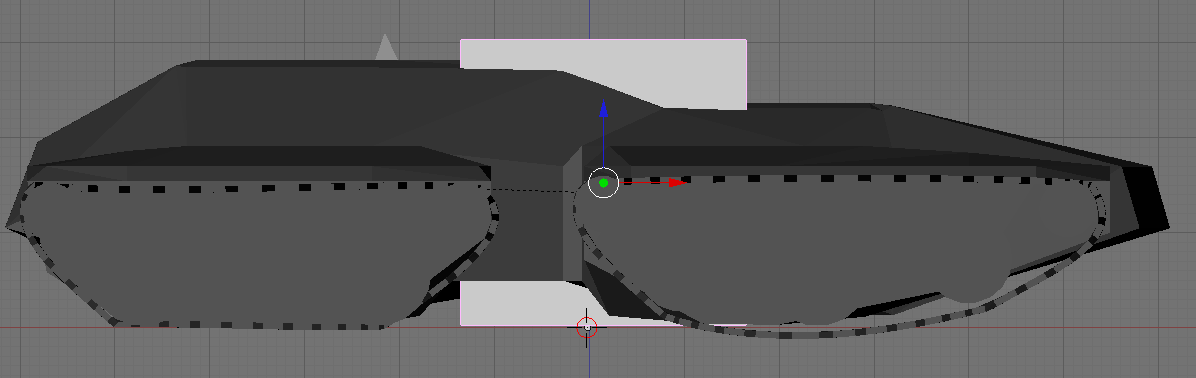
\includegraphics[width=0.50\textwidth]{Figures/tankAndCube.png}
	\caption{A tank and  x15 scale cube}
	\label{fig:Scale Sample}
\end{figure}


\subsubsection {Modelling Tips and Tricks}
Very good blender tutorials can be found in the \href{http://en.wikibooks.org/wiki/Blender_3D:_Noob_to_Pro}{Blender Noob to Pro Tutorials}.

\subsubsection {Naming Conventions}
\textit{Mesh Conventions}

Mount : This is the position where an object that is attached to the current mesh will be placed. See the pyramid where the turrent will be attacehd to the tank in Fig 3.1.

Color : Any mesh named Color will change color depending on the player's settings.

Cannon0 : The gun barrels should be named Cannon0. For multiple cannons start with Cannon1, Cannon2 etc.

Emitter0 : This is the position where projectiles will be generated from a mesh. For multiple emmitters user Emitter1, Emitter2 etc. 

\textit{Model Conventions}

The name that you give a model will be the name of the unit in game (eg. Behemoth.fbx is the model for the Behemoth tank) so choose your names accordingly. Also, every tank or weapon should have an associated \_dead model that will display when the entity is destroyed in game. These should be named MODELNAME\_dead.fbx (eg. Behemoth\_dead.fbx).

\textit{Texture Conventions}

Be as specific as possible with your texture names. Follow the example modelname\_meshname\_texturename.png, where 'modelname' is the name of the associated .fbx file (ex. Cannon), 'meshname' is the name of the specific mesh this texture will be applied to (ex. GunBarrel0), and 'texturename' is a description of the type of texture (ex. Forestgreen\_Rusted).


\subsubsection {Texturing}
XNA only supports UV texturing. UV involves making seams in your mesh so that blender can cut along then and unwrap your 3d mesh onto a 2d surface. You then draw an image or upload and image onto this surface. Blender will map the image to your model with respect to the faces in the unwrapped mesh. This sounds complicated but is actually very easy.

\begin{enumerate}
	\item Apply a different material to every part of model that requires a different texture.
	\item Right click on top of viewing panel and select 'Split Area'.
	\item Select 'UV / Image editor' from the box in the lower left corner of the new window.
	\item In the original window, select the part of your model you want to texture on and enter Edit Mode.
	\item Select the edges that you want Blender to use as seams, press 'CTRL + E' amd select 'Mark Seam'.
	\item Select entire area, press 'U' and select 'Unwrap'. The 'UV / Image editor' window should now display a flattened version of your model.
	\item Edit the flattened image until you are ready to draw on it. Keep in mind that highly visible areas on your model should not have seams and similar sized polygons in 3D should be represented by similar sized polygons in 2D.
	\item Export the 2D wireframe by following 'UVs / scripts / Save UV Face Layout'.
	\item Create a texture using the wireframe as a reference in an image editor. Note: Image size must be a power of 2 (ie. 256, 512 and 1024).
	\item Import your image in the UV editor by following 'Image / Open'.
\end{enumerate}

You are done. Preview your texture by changing the viewpoint shading to Textured in the 3D object window. 

Note: If you move the verticies or change the model after importing an image you will probably need to re-export the 2D wireframe and remake the texture.

Follow these steps for each other area you want to texture.

\subsubsection {Exporting for VTank}
Your model must follow a specific set of rules in order to display correctly in VTank. Be aware that 'Main' mesh refers to the main body of your model and not a mesh named Main.

\begin {enumerate}
\item {\bf Your model conforms to the Orientation, Scale, Naming, and Texturing protocols. }
\item {\bf Your model has no change in Scale or Rotation from it's ObDATA. }\\
\begin{itemize}
	\item Enter 'Object mode'
	\item Select all objects by pressing 'A'
	\item Pess 'CTRL + A' and select 'Scale and Rotation to ObData'
\end{itemize}

Note: If you rotate or scale your model again, you must repeat this step. 

\item {\bf The main mesh's center is placed correctly.Y}\\
Placing the center is very important, as it is the point that your model will rotate around while moving in game. It also defines where the model will rest on the ground. Keep this in mind when placing your centers. 

Method 1: 
\begin{enumerate}
	\item Go to 'Object Mode'.
	\item Select your main mesh and enter 'Edit Mode'.
	\item In 'Editing Panel' (F9) go to 'Mesh / Center New'.
	\item Select 'Object / Snap / Cursor to Selection'.
	\item Go to 'Object Mode'.
	\item Without moving the cursor, select 'Add / Mesh / Empty Mesh'.
	\item Reposition the empty mesh so it is level with the bottom of the model.
	\item Select the main mesh press 'Shift' and select the empty mesh.
	\item Press 'CTRL + J' and then 'Enter'.
	\item Rename the main mesh to it's original name.
\end{enumerate}

Note: Keep in mind that this method puts the center at the location of the empty mesh. This might not be exactly where you want your model to rotate. Use your best judgment. 

Method 2: The previous way makes it easier to place your center in the right place if your mesh is relatively balanced. Another way to place your center is to get your cursor where you want your center to be and then select your main mesh, enter 'Edit Mode', open the 'Editing Panel'(F9) and go to 'Mesh Panel / Center Cursor'. This will place the objects new center wherever you placed your cursor. You can use the 'Object / Snap' functions to make this a lot easier.

Note: Remember to re save your ObData!

\item {\bf The center for your 'Main' mesh is at the origin.}\\
Now that your model has a correct center, move your entire model so the center is at the origin of Blender's grid. Again, this is easily done with the 'Object / Snap' functions. 

\item {\bf All meshes in your model are somehow connected.}\\
Usually using the add parent function. To add a parent, first make sure that all of the meshes are in the right place and the ObData is saved, then go to object mode. Select the object that you want to make the child, then hold ShiftKey and select the object to make the parent. Now press CntrlKey+PKey and click Add Parent. 

Note: If you change anything after setting the parent you must UnParent before resaving the ObData. Do this by selecting all objects, pressing AltKey+PKey and selecting Clear Parent (Save Track).

Note: Remember to resave your ObData!

\item {\bf Export}\\
When ready, go to  File / Export / Autodesk FBX (.fbx) Modified for XNA. A box will appear. Select 'Scene Objects' and deselect 'X90'. Click export. Choose the name for your file and its destination folder and click 'Export FBX'. Make sure the export 
\begin{figure}[h]
	\centering
		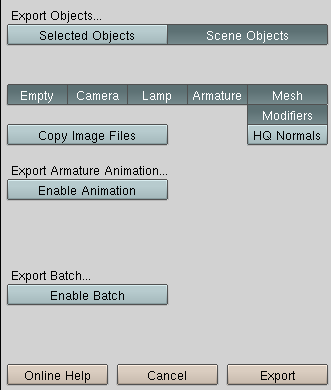
\includegraphics[width=0.50\textwidth]{Figures/ExportFBX.png}
	\label{fig:ExportFBX}
\end{figure}


\item {\bf Double Check .fbx File}\\
Sometimes, the links to your textures in the .fbx file are not correct. To fix this open the .fbx file in a text editor and search for the texture names with CtrlKEY+FKEY. Make sure that the path to the texture is correct and the texture and .fbx files are in the right place. 

\end{enumerate}

\section{Dynamic Model Viewer}

The dynamic model viewer is a tool created by the VTank team that is used by artists who want to see what their creations will look like in game without writing any code. Available in the VTank.sln file, just build it and run it. 


\begin{table}[h]
	\centering
		\begin{tabular} {l | r}
		C & Toggle camera views \\
		S & Toggle shadows \\
		L & Toggle lighting \\
		Num+ & Change percentage of day complete \\
		E & Deploy previously loaded particle emitter \\
		Ctrl + T & Load a tank model \\
		Ctrl + W & Load a weapon model \\
		Ctrl + P & Load a power up model \\
		Ctrl + E & Load a particle emitter \\
		Ctrl + A & Load an animated model \\
		Ctrl + O & Load any other model \\
		Left or Right & Rotate a Tank model \\
			
		\end{tabular}
\end{table}

The differences between loading model types only deals with how they are positioned. For instance, loading a tank and a turret will automatically attach the turret to the tank and loading a powerup will draw the model above the ground. Tanks and turrets will also vary the mesh color to show how they might look in game. 

To load a particle emitter you must load two files. The first is a particle system settings file (*.vtpss) and the second is a particle emitter settings file (*.vtpes). Also note that the texture image that the emitter uses must be a part of the project.  

\section{Map Previewer}

The map previewer is another tool created by the VTank team that enables users to preview what a map looks like ingame.  It was created to make up for the fact that our map editor only represents 2d tiles an icons, which do not adequately convey a map's actual appearance.  The map previewer puts you behind a cactus model, and allows you to 'drive' around a given map, inspecting what it looks like, without having to upload it to the active map rotation.

The controls are similar to VTank controls, with a few differences.

\begin{table}[h]
	\centering
		\begin{tabular} {l | r}
		F & Load a Map \\
		W & Forward \\
		A & Rotate Left \\
		S & Backward \\
		D & Rotate Right \\
		Spacebar & Toggle Chase / Overhead \\
		Up Arrow & Tilt Up \\
		Left Arrow & Tilt Left \\
		Right Arrow & Tilt Right \\
		Down Arrow & Tilt Down \\			
		\end{tabular}
\end{table}

Note that a map can be loaded again without closing the map previewer, enabling you to continue working on your map in \MapEditor, and reload the map when you want to see your changes.

Unfortunately, the map previewer is not associated with the main VTank project, but it can be downloaded freely from the \href{http://vtank.cis.vtc.edu/downloads}{VTank Website}, just below the download for \MapEditor.